\chapter{Implementation Details}
    \label{implementation}

After having transformed the acquired data into a usable format, the fish's anatomy can be modelled. The whole implementation process was done in python \cite{van1995python} using version 3.7.0. The details of that implementation process are explained in this chapter. First, a simplex optimisation was applied to the parameters describing the edited ellipses that approximates the ellipses. Subsequently, the backbone and its relative position to the created cross-sections were defined depending on the fish's curvature. Once this information was gained, a polynomial regression was applied to the parameters describing the cross-sections contours. This process is described in the third section followed by a description of the resulting final function. That same function classifies points according to their position relative to the fish.

\section{Simplex Optimisation on Cross-sections}
    \label{simplex}
    
In order to fit the function described in equation \ref{eq:ellipsis} to the cross-section contours resulting from the transformations in the previous section, an appropriate optimisation method is needed. As the simplex optimisation method \cite{nelder1965simplex} does not assume any premises and works with higher amounts of free variables and nonlinear problems, this is the method we used to find the optimal parameter values for $a,b$ and $m$ for each section. 

As a starting point, the simplex downhill method for unconstrained problems needs $n+1$ points in $n$-dimensional space to form a convex combination of these points. In our case, $n$ is 3 because of the three variables $a,b$ and $m$ that need to be optimised. The point's convex combination is called simplex and gives the method its name. One step is executed by first evaluating all points according to a given error function which is meant to be minimized. For our problem, the error function is based on the distance from the origin to a point on the contour with angle $\varphi$, let us name it $d(\varphi)$. This value is then compared to the fitted value with given parameters $a,b$ and $m$ in $r(\varphi)$ (see equation \ref{eq:ellipsis}) for all existing points and the corresponding $\varphi$-values:
\begin{flalign}
err(a,b,m) = \sum_{all \textit{ } \varphi}{\abs{d(\varphi)-r(\varphi)}}.
\end{flalign}

The next step in the optimisation process is to choose the point for which $err(a,b,m)$ is highest, meaning that this point, let it be called $p_0$, is the worst choice of parameters. $p_0$ therefore gets replaced by a new point $p_{new}$ that is created by projecting $p_0$ through the center of the hyperplane spanned by the other points to the other side. A new simplex with a convex combination of the new point and the remaining old points is the result. This process is repeated until the error function converges indicating a local or global minimum. 

To reduce the probability of ending in a local minimum, we applied the simplex algorithm implemented in the scipy-package \cite{2020SciPy-NMeth} ten times with random starting values (in given intervals: $a \in [-50,50], b\in [-50,100], m \in [-20,20]$) for the first section. The intervals were chosen after manual tests with various starting values whose maximal and minimal values are included in this range. After having found parameter values minimizing the error for the first section, these values were passed over to the next call of the simplex function for the following section and so on. This repeated passing over has been done because we assumed that the optimal parameters do not change a lot between consecutive sections. 

The overall squared error, meaning the added error over all sections (60), was 63,244,722 px$^2$ which is a mean squared error of $1026.68$ px$^2$ per section. One example of a fitted cross-section and the corresponding cross-section points can be seen in Figure \ref{fig:fitted_ellipsis}. Figure \ref{fig:ellipses} assembles the fitted cross-sections in three dimensions to give a better impression of the resulting fish.

\begin{figure}
    \centering
    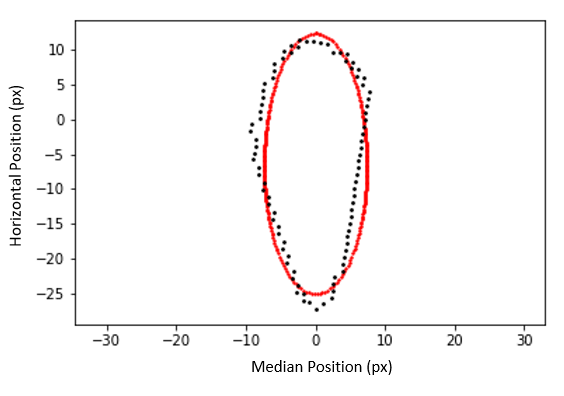
\includegraphics[width = 0.75\textwidth]{figures/FittedEllipsis_64.png}
    \caption{Depicted in red are the fitted cross-section's contour to the cross-section's transformed MRI data (points in black) of a section positioned relative close to the center of the fish's long axis (64 mm caudal to the fish's head). The points in this figure have already been centered on the backbone's position. How this was done exactly is described in chapter \ref{Backbonecoordinates}. One can see clearly, that the tipped edge at the ventral side in the original data is not approximated well by the fitted ellipsis and this holds for all pictures including a tipped edge. }
    \label{fig:fitted_ellipsis}
\end{figure}

\begin{figure}
    \centering
    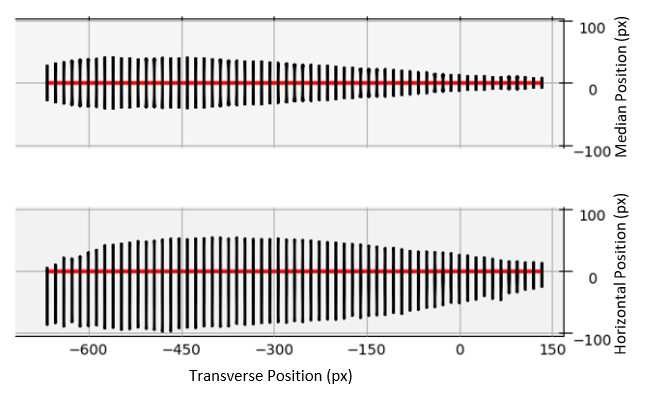
\includegraphics[width = 1\linewidth]{figures/Ellipses.PNG}
    \caption{Ellipses resulting from simplex optimisation (in black) positioned next to each other along the backbone (in red), once as seen from above the fish (upper figure), once as seen from beside the fish (lower figure).}
    \label{fig:ellipses}
\end{figure}


\section{Backbone Coordinates}
    \label{Backbonecoordinates}

To be able to transform the sections from two to three dimensions, the implementation of the backbone itself needs to be done. 

The implementation of the hyperbola modelling the backbone is done straightforward from the mathematical model described in chapter \ref{BackboneModelling}. $f(x)$ is implemented, depending on $\theta$, the angle between x-axis and the second asymptote, and $d$, the intersection with the $y$-axis. 

However, the calculation of $s^{-1}(l)$ cannot be done easily as $s(x)$ is not always a strict monotonic function (for negative $x$-values the curve is a constant function with $y=0$ for most $\theta$ and $d$ values). However, strict monotony would be necessary for building the inverse function. Therefore, the calculation of $s^{-1}(l)$ is replaced by a look-up table with 10000 entries ($x \in [Head, Head + 120]$, $l \in [0, s(Head+120)]$). Searching for a given $l$ in that same look-up table results in a value close to the exact inverse value, $s^{-1}(l)$. The search is done via a binary search that has a running time of $O(log(n))$ with $n$ being the number of entries in the look-up table. 

As the next step, the cross-sections need to be positioned correctly relative to the now existing backbone-coordinates. Therefore, the contours are supposed to be centered around the backbone's position and not around its center of mass like previously. Hence, a translation in horizontal directions needs to be executed according to each section's position relative to the backbone. 

As described in chapter \ref{preprocessing}, the coordinates of the backbone have been included in the convex hull picture and could therefore be determined later on in the second edge image. Its median coordinate is not relevant because of the fish's symmetry in median direction. In contrast, the horizontal coordinate is the source used to determine the necessary translation called \textit{x\_offset} in the further descriptions and also in our code (see supplementary material). A translation for the determined sections could be done easily with the detected backbone positions, but only for the discrete positions on the backbone at which the sections are located and only for sections located caudal to the swim bladder. However, we need to be able to calculate the \textit{x\_offset} at each point $l$ on the backbone. Thus, a polynomial regression with a degree of two was applied to the detected positions to predict the missing positions. The $R^2$ value for that model is 0.95 and is thus providing a sufficient fit. The model is depicted in Figure \ref{fig:paramreg} at the right bottom.

The backbone's positions can be approximated for any $l$ with the resulting function. Hence, the fitted contours can be positioned relative to the backbone in the two-dimensional space.

\section{Ellipses Parameter Regression}
    \label{parameterregression}
    
Additionally to the polynomial regression for the \textit{x\_offset}, polynomial regressions were applied to the parameters $a,b$ and $m$ which resulted from the simplex optimisation. The reason for these additional regressions are the jumps that can be seen in Figure \ref{fig:fitted_ellipsis} that may be caused by inaccuracies in previous transformation steps. $a$ and $b$ are well predictable with a polynomial regression of degree 3 as their $R^2$ values are 0.99 and 0.93, accordingly. In contrast, $m$, the parameter for defining the contour's tip at the bottom, does not seem to be describable by a polynomial model, at least not with degree 3 ($R^2 = 0.46$). But even with a degree of ten, the fit does not get significantly better. All those regressions are depicted in Figure \ref{fig:paramreg}. 

The resulting smoothed fish in three dimensions is visualized in Figure \ref{fig:ell_regression}.

\begin{figure}
\centering
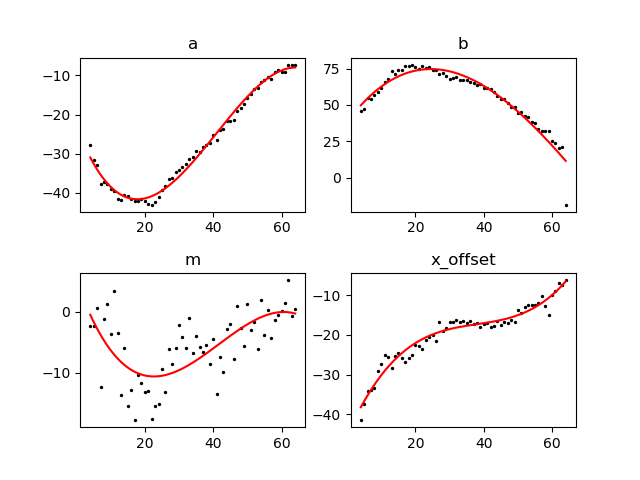
\includegraphics[width = 1\linewidth]{figures/param_regressions.png}
\caption{The four figures show the values for $a,b,m$ and the \textit{x\_offset} given by simplex optimisation for the existing cross-sections from the MRI data (points in black). The red lines each show the results of the polynomial regressions with degree 3 over the fitted values separately for $a,b,m$ and the \textit{x\_offset}.}
\label{fig:paramreg}
\end{figure}

\begin{figure}
\centering
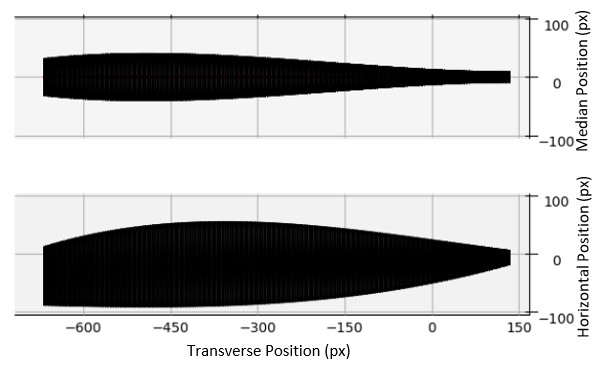
\includegraphics[width = 1\linewidth]{figures/Ellipsis_regression.png}
\caption{Smoothed ellipses with parameters $a$,$b$,$m$ and  $x\_offset$ resulting from the polynomial regressions over each parameter put together along the backbone to form the fish's body. The upper picture shows the resulting fish's contour as seen from above the fish, the picture at the bottom as seen from aside.}
\label{fig:ell_regression}
\end{figure}


\section{Fish-discrimination Function}
    \label{finalfunction}

The purpose of the final function is to describe a point's position relative to the fish. Is the point located outside the fish or inside? If the latter is the case: is it positioned within the backbone, the spinal chord or the electric organ? These five categories should be distinguished from each other to then be able to model the fish's electric field and the response of its electroreceptors precisely. \\

\subsection{Definition of the Closest Point}
    \label{closestpoint}
The first step towards a categorization of a point $p_W$, given in world coordinates, is calculating the point $l$ on the backbone to which $p$ has the smallest distance. To do so, the following distance function is defined based on the backbone's definition. $P$ is the point for which its position needs to be determined, $P_B$ is a point on the backbone described only by the $x-$coordinate.

\begin{flalign}
||P-P_B|| = \sqrt{(p_x-x)^2 + (p_y-\frac{1}{2}(ax + \sqrt{4d^2 + a^2x^2})^2 + p_z^2}
\end{flalign}

The distance function depends solely on $x$ and therefore one can take its derivative and set it to zero to get the $x$-value for which it is minimal, $x_0$. This was done in python using the sympy differentiation and solve methods \cite{sympy2017}. Having evaluated $x_0$, the calculation of $l$ follows straightforward from \ref{eq:s_x}.

The tangential vector of $l$, described as $\vec{e_1}$ in previous paragraphs, is then orthogonal to the vector between $l$ and $p$ because the orthogonal distance is always smaller than non-orthogonal distances \cite{ahn2002orthogonal}. Points having their closest point $l \not \in [0,120]$ can be directly labeled as outside the fish as long as the bent of the fish's tail is not positioned very close to the tail's endpoint. If that happens, it may lead to a corresponding point $l$ cranial to the fish's tail while another perpendicular point $l_0$ is positioned caudal to the tail although it is further away. Still, it would then be possible that the point to be categorized is localized within the fish, because the distance to $l_0$ is smaller then the threshold at this point. The described position of the fish with a bent of the tail really at the end of the fish is not something that is interesting for research purposes. As described in section \ref{BackboneModelling}, the standard exploration behaviour is executed with a bent approximately at the fish's center close to the transverse section. The boundaries for points being possibly inside or definitely outside the fish, are depicted in Figure \ref{fig:borders}.

The orthogonality property for points being possibly inside the fish has been used to test the result from the calculations so far via the scalar product. For 150 tested points the maximal scalar product was 0.0688. It is not exactly zero because of inaccuracies following from the look-up table evaluating $s^{-1}(x)$.

\begin{figure}
    \centering
    \includesvg[width = 0.85\linewidth]{figures/outer_borders.svg}
    \caption{Points being labeled as inside or outside the fish according to the illustrated boundaries. The figure shows the fish's backbone in a curved position (black line; $\theta = 60, d = 4, Head = -70$) from head to tail and its theoretical further development before the head and behind the tail (dashed lines). The outer boundaries (dotted lines) determine whether points are possibly inside the fish or outside, at this point not depending on their distance to the backbone but only on their corresponding point $l$ on the backbone which has the closest distance to the given point. Points to the left of the left boundary do have a closest point $l$ on the backbone smaller than $0$, points to the right of the right boundary fulfil $l>l(Tail)$. The bend of the right border is caused by the bend of the backbone because points located higher than the border's bend possibly have two points on the backbone with an orthogonal tangential vector. One then needs to distinguish between the points being closer and further away and that is done according to the vertical part of the right border.}
    \label{fig:borders}
\end{figure}


\subsection{Relative Position to the Fish}
    \label{relativeposition}
Having calculated the closest point $l$ on the backbone, the next step for determining $p$'s position is getting its position relative to that same point l. To achieve this, one needs to transform ${}^Wp$, given in world-coordinates, by ${}^LT_W$, where $L$ describes the coordinate frame centered on $l$. Therefore, the inverse of ${}^WT_L$ needs to be calculated and then multiplied with $p$. It is
\begin{flalign}
{}^WT_L = \begin{pmatrix} cos(\varphi) & -sin(\varphi) &0 & l_x \\
sin(\varphi) & cos(\varphi) & 0 & l_y \\
0&0&1&0 \\ 0&0&0&1\end{pmatrix}
\end{flalign}
with
\begin{flalign}
\varphi = cos^{-1}\left(\vec{e_1} \cdot \begin{pmatrix}
1 \\ 0 \\ 0 
\end{pmatrix}\right).
\end{flalign}
No normalization is needed here, because both $\vec{e_1}$ and the $x$-axis unit vector do have a norm of 1.
Calculating the inverse of that matrix and applying it to ${}^WP$ results in:
\begin{flalign}
{}^LT_W \cdot {}^WP = \begin{pmatrix} cos(\varphi) & sin(\varphi) &0 & -l_x\cdot cos(\varphi) - l_y \cdot sin(\varphi) \\
-sin(\varphi) & cos(\varphi) & 0 & l_x \cdot sin(\varphi) -l_y\cdot cos(\varphi) \\
0&0&1&0 \\ 0&0&0&1\end{pmatrix}
\cdot
\begin{pmatrix}
p_x \\ p_y \\p_z \\1
\end{pmatrix}
= {}^LP.
\end{flalign}

Then ${}^LP$ is of the form
\begin{flalign}
{}^LP= \begin{pmatrix}
\tilde{p_x} \\  \tilde{p_y} \\ p_z \\1
\end{pmatrix}
\label{eq:l_p}
\end{flalign}

with

\begin{flalign}
\tilde{p_x} = (p_x-l_x) \cdot cos(\varphi) + (p_y - l_y) \cdot sin(\varphi) \\
\tilde{p_y} = (l_x-p_x) \cdot sin(\varphi) - (l_y-p_y) \cdot cos(\varphi).
\label{eq:py}
\end{flalign}

The tangential vector $\vec{e_1}$ of $l$ can be written as

\begin{flalign}
\vec{e_1}=\begin{pmatrix}
cos(\varphi) \\ sin(\varphi) \\ 0
\end{pmatrix}
\end{flalign}

$\vec{lp}$ by definition is

\begin{flalign}
\vec{lp} = \left(\vec{p} - \vec{l}\right) = \begin{pmatrix}
p_x - l_x \\ p_y - l_y \\ p_z - l_z
\end{pmatrix}.
\end{flalign}

Because of the perpendicular arrangement of $\vec{e_1}$ and $\vec{lp}$, it holds

\begin{flalign}
\langle \begin{pmatrix}
p_x - l_x \\ p_y - l_y \\ p_z - l_z
\end{pmatrix},
\begin{pmatrix}
cos(\varphi) \\ sin(\varphi) \\ 0
\end{pmatrix}
\rangle = 0
\iff (p_x - l_x) \cdot cos(\varphi) + (p_y - l_y) \cdot sin(\varphi) = 0.
\end{flalign}

As this is equivalent to $\tilde{p_x}$, the $x$- coordinate of ${}^LP$ is always zero. $p_z$ does not change, as $l_z$ is always zero. Following from that, there is no translation in $z$-direction no matter the exact values of $p$. That results in

\begin{flalign}
{}^LP= \begin{pmatrix}
0 \\ \tilde{p_y} \\ p_z
\end{pmatrix}.
\end{flalign}

To be able to decide, whether $p$ is located inside the fish, one needs to compute the threshold for the resulting angle between ${}^LP$ and the origin. The fitted ellipses were constructed not relative to the position of the backbone but to the backbone translated by the corresponding \textit{x\_offset}, let us name that point $b_0$. Therefore, the angle and distance of ${}^LP$ need to be calculated relative to $b_0$, as well. Translating $p$ by the \textit{x\_offset} and then calculating both values has the wanted effect. Hence, this is what has been done:
\begin{flalign}
d_p &= \sqrt{\tilde{p_y}^2 + (p_z +x\_offset)^2}\\
{}^L\tilde{P} &= \begin{pmatrix}
\tilde{p_y} \\ p_z + x\_offset
\end{pmatrix}, \vec{e_x} = \begin{pmatrix}
1 \\ 0 
\end{pmatrix}\\
\theta &= cos^{-1}\left( \frac{{}^L\tilde{P}\cdot \vec{e_x}}{||{}^LP'\cdot \vec{e_x}||}\right).
\end{flalign}

Using the coefficients from the parameter regression described in section \ref{parameterregression}, it is possible to calculate the exact parameters for the determined $l$-value. Substituting these parameters and the angle $\theta$ into equation \ref{eq:ellipsis} leads to the distance from $b'$ to the point on the contour with the same angle. Thus, this value specifies the threshold for categorizing a point as inside or outside the fish. Comparing this threshold to $d_p$, the categorization inside/outside is complete. The fish resulting from all points being labeled as inside can be seen in Figure \ref{fig:final_fish}.

\begin{figure}[ht] \label{ fig7} 
\captionsetup[subfigure]{labelformat=empty}
  \begin{subfigure}[b]{0.5\linewidth}
    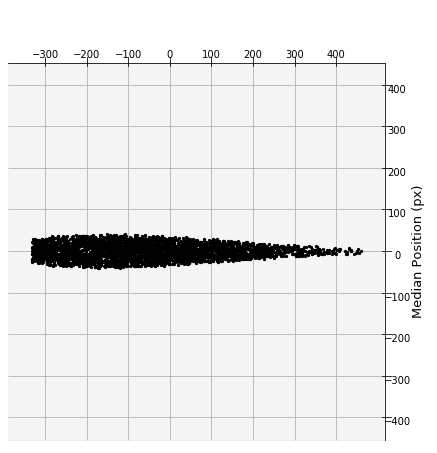
\includegraphics[width = 1 \linewidth]{figures/final_fish_straight_median.PNG} 
  \end{subfigure} 
  \begin{subfigure}[b]{0.5\linewidth}
    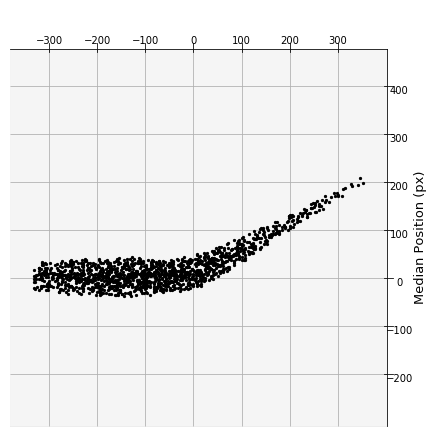
\includegraphics[width = 0.99 \linewidth]{figures/final_fish_turned_median.png} 
  \end{subfigure} 
  \begin{subfigure}[b]{0.5\linewidth}
    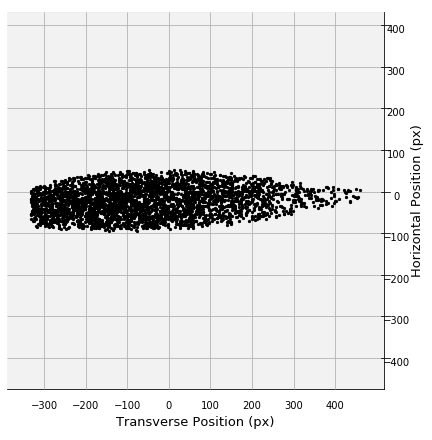
\includegraphics[width = 1\linewidth]{figures/final_fish_straight_horizontal.PNG} 
  \end{subfigure}
  \begin{subfigure}[b]{0.5\linewidth}
    %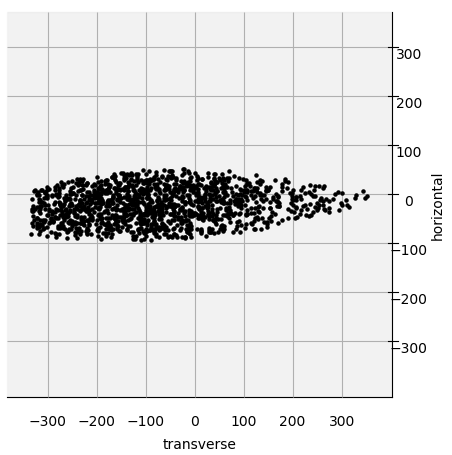
\includegraphics{figures/final_fish_turned_30_2_minus50_10000_1.png} 
    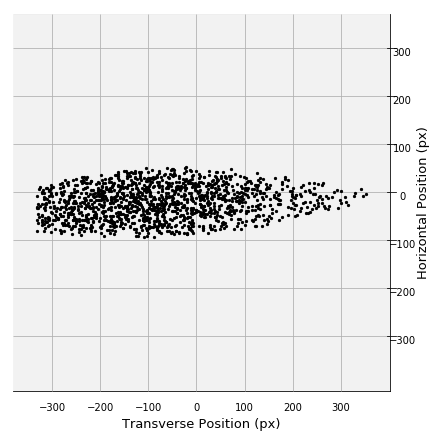
\includegraphics[width = 1.02\linewidth]{figures/final_fish_turned_horizontal.png}
  \end{subfigure} 
  \caption{On the left, one can see all points of 10000 random points within a range of $Head$ to $Tail$ in transverse direction, $-100$ to $100$ in median direction and $-50$ to $50$ in horizontal direction labeled as inside the straight fish ($\theta = 0, d = 0, Head = -50 \cdot (1/0.15)$) by the final function. The top graphic shows the fish as seen from above, the bottom one as seen from aside (see \ref{fig:ell_regression} for comparison). On the right, the same can be seen for a fish with values of $\theta = 30, d = 2$ and $Head = -50 \cdot (1/0.15)$ and 10000 points within the ranges of $Head$ to $Tail$, $-50$ to $220$ and $-100$ to $60$, respectively. Less points are labeled as being inside for the turned fish because the median range is a lot wider than for the straight fish.}
  \label{fig:final_fish}
\end{figure}

\subsection{Categorization within the Fish}
    \label{innerparts}
    
Next, the differentiation of the considered inner parts can be done. This further differentiation is only necessary, of course, for points categorized as being on the inside of the fish. 

First, we want to consider the backbone. Measured on various MRI pictures, the backbone seems to have a constant radius $r_b$ of about $0.415$ mm. It is observable on picture 34 and all pictures caudal to that one. The straightforward classification for points positioned inside the backbone therefore is based on these two criteria: Is the distance of ${}^LP$ (without the translation of \textit{x\_offset}) smaller than $r_b$? And, secondly, is the corresponding $l$ positioned caudal or at the corresponding position of cross-section number 34? 

Second, points located inside the spinal chord should be labeled as such. The radius of the spinal chord, $r_s$, being $0.466$ mm is constant throughout the whole fish. It is also visible in pictures caudal to the $34^{th}$ picture. As it can be seen in Figure \ref{fig:innerparts}, there is no distance between spinal chord and backbone. At least, it is too small to detect in the MRI scan, if present. A translation of the point by $r_s+r_b = 0.881$ mm in ventral direction and a calculation of this point's distance to the origin is equivalent to calculating the point's distance directly to the spinal chord's center. Again, the two criteria need to be fulfilled in order to classify a point as positioned inside the considered part, in this case the spinal chord. 

Third, it needs to be verified if the given point is located within the electric organ or not. As depicted in Figure \ref{fig:innerparts}, the electric organ was modelled by two mirrored triangles ventral to the backbone. The offset between the backbone's center and the triangles' left/right tip is termed \textit{e\_offset} and varies along the backbone. It is visible in a triangular form on the MRI images only in sections 50 and the ones caudal to it. Cranial to that, it is visible until the cranial end of the swim bladder but its form is different. Due to time constraint, this part of the electric organ has not been included into the implementation. For the included part, primarily, one needs to define \textit{e\_offset} and \textit{width}, distance between left and right tip of the electric organ, at each point of the backbone. To do so, two linear regressions were performed using three values at three different section as a basis (one for the \textit{width}, one for the \textit{e\_offset}). The resulting $R^2$ values suggest that the models fit well: $R^2_{width} = 0.9998, R^2_{e\_offset} = 0.9836$. The fitted coefficients and intercepts were then used to define width and e\_offset at each point $l$. The application of the following formulas then leads to the position of the triangles vertices.
\begin{flalign}
\frac{\gamma}{2} &= \sin^{-1}\left({\frac{0.5 \cdot c}{b}}\right) \\
A &= \begin{pmatrix}
\pm 0.5 \cdot width \\ -e\_offset
\end{pmatrix}\\
B &= \begin{pmatrix}
A_x \pm b \cdot \cos\left(\frac{\gamma}{2}\right) \\ A_y -b \cdot \sin\left(\frac{\gamma} {2}\right)
\end{pmatrix}\\
C &= \begin{pmatrix}
A_x\pm \cdot \cos\left(\frac{\gamma}{2}\right) \\A_y +b \cdot \sin\left(\frac{\gamma} {2}\right)
\end{pmatrix}.
\end{flalign}
With that, one can calculate whether a point is positioned within one of the two triangles. One way to do that is to transform the given point into the barycentric coordinate system \cite{farin2008mathematical}. Hence, the point is written as a linear combination of the vertices $A,B,C$: $ P = s \cdot A + t \cdot B + u \cdot C$ with 
\begin{flalign}
s = \frac{area[P, B, C]}{\mathcal{A}}\\
t = \frac{area[P, C, A]}{\mathcal{A}}\\
u = \frac{area[P, A, B]}{\mathcal{A}}
\end{flalign}
 where $\mathcal{A}$ describes the triangle's area and thus $\mathcal{A} = area[A,B,C]$. 
 
 In two dimensions it holds: $s+t+u = 1$, no matter where $P$ is positioned. Additionally, if $P$ is located within the triangle, it follows that $s,t,u \geq 0$. This property can be used to test whether a given point is located within or outside a triangle.
 
The described process was implemented and builds the second condition for a point being located within the electric organ alongside with the point being positioned closest to a point $l$ on the backbone corresponding to a section $\geq 50$. 

\begin{figure}
    \centering
    \fbox{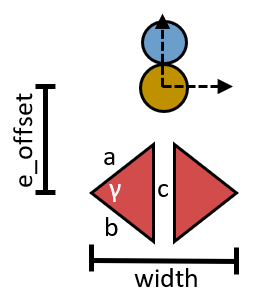
\includegraphics{figures/Crosssectionmodel.PNG}}
    \caption{This illustrations depicts a simplified version of the considered parts in the interior of the fish. The backbone is depicted in yellow below the spinal chord (blue). The electric organ is shown in red, its offset is marked on the left. It is measured from the electric organ's tip to the center of the backbone. The width specifies the width between the two tips of the electric organ.}
    \label{fig:innerparts}
\end{figure}

In conclusion, a given point is label as 'outside','inside', 'backbone', 'spinal chord' or 'electric organ'. The resulting labels for points located closest to the same $l$ is depicted in Figure \ref{fig:sectionlabel}.

\begin{figure}
    \centering
    \includesvg[width = 0.8\textwidth]{figures/labeling_section29.svg}
    \caption{Labeling of 10000 points within a range of $-50$ to $50$ mm on the median axis and $-100$ to $60$ mm on the horizontal axis in the paratransverse section located $58$ mm caudal to the fish's head. Points in red are classified as outside the fish, points in yellow are classified as being on the spinal chord, points on the backbone are depicted in violet and points in green are located within the electic organ. Points classified as inside the fish are not included for enhanced clarity of the inner part labels.}
    \label{fig:sectionlabel}
\end{figure}






